
% MORGAN STANLEY RESEARCH - siRNA THERAPEUTICS REPORT
% Following LaTeX Style Guide conventions

\documentclass[10pt, a4paper]{article}
\usepackage[a4paper, top=2.2cm, bottom=2.5cm, left=1.4cm, right=1.4cm, headheight=1.5cm]{geometry}
\usepackage[T1]{fontenc}
\usepackage[scaled]{helvet}
\renewcommand{\familydefault}{\sfdefault}

\usepackage[table]{xcolor}
\usepackage{graphicx}
\usepackage{tcolorbox}
\usepackage{booktabs}
% \usepackage{colortbl} % Removed to prevent conflict
\usepackage{array}
\usepackage{tabularx}
\usepackage{fancyhdr}
\usepackage{tikz}
\usepackage{pgfplots}
\usepackage{float}
\usepackage{caption}
\usepackage{multicol}
\usepackage{adjustbox}
\usepackage{titlesec}
\usepackage{enumitem}
\usepackage{hyperref}

% Hyperref setup for clickable TOC
\hypersetup{
    colorlinks=true,
    linkcolor=msblue,
    urlcolor=msbrightblue,
    citecolor=msblue,
    pdftitle={siRNA Therapeutics: The Next Frontier in Precision Medicine},
    pdfauthor={Morgan Stanley Research},
}

% Fix for array/colortbl compatibility issue with p columns
\makeatletter
\let\insert@pcolumn\insert@column
\makeatother

% --- BRAND COLORS ---
\definecolor{msblue}{HTML}{002A5C}       % Morgan Stanley Dark Blue
\definecolor{msbrightblue}{HTML}{0096D6} % Light Blue for "INSIGHT" and Highlights
\definecolor{msgrey}{HTML}{F2F2F2}       % Light Grey for Backgrounds
\definecolor{mstextgrey}{HTML}{666666}   % Grey text for analysts
\definecolor{mstableheader}{HTML}{E5E5E5} % Grey for table headers

% --- PAGE HEADER/FOOTER ---
\pagestyle{fancy}
\fancyhf{}
\renewcommand{\headrulewidth}{0pt}

% Left Header: Logo
\lhead{
    \vspace{0.2cm}
    {\fontsize{14}{14}\bfseries Morgan Stanley} 
    \hspace{0.15cm} \textcolor{black}{|} \hspace{0.15cm} 
    {\footnotesize\bfseries RESEARCH} \\
    {\color{mstextgrey}\footnotesize \today}
}

% Right Header: Region/Type
\rhead{
    \vspace{0.2cm}
    {\color{msbrightblue}\bfseries\small GLOBAL HEALTHCARE INSIGHT}
}

% Footer
\lfoot{\color{mstextgrey}\footnotesize Morgan Stanley Research}
\rfoot{\bfseries\thepage}

% --- TYPOGRAPHY & SECTIONS ---
\titleformat{\section}
  {\color{msblue}\normalfont\Large\bfseries}{}{0em}{}
  
\titleformat{\subsection}
  {\color{black}\normalfont\large\bfseries}{}{0em}{}

% --- CUSTOM COMMANDS ---

% 1. Report Title Block
\newcommand{\reporttitle}[3]{%
    \vspace{0.5cm}
    {\fontsize{14}{16}\selectfont\color{msbrightblue}\bfseries #1 \par} % Ticker/Company
    \vspace{0.1cm}
    {\fontsize{28}{32}\selectfont\color{black}\fontseries{l}\selectfont #2 \par} % Main Title
    \vspace{0.5cm}
}

% 2. "What's Changed" / Estimates Table
\newcommand{\estimatesbox}[1]{%
    \begin{tcolorbox}[colback=msgrey, colframe=white, boxrule=0pt, sharp corners, left=2pt, right=2pt, top=2pt, bottom=2pt]
    \textbf{\footnotesize WHAT'S CHANGED}
    \end{tcolorbox}
    \vspace{-0.3cm}
    #1
    \vspace{0.5cm}
}

% 3. Sidebar Analyst Info
\newcommand{\analystinfo}[3]{%
    {\bfseries\small #1} \\
    {\color{mstextgrey}\tiny #2} \\
    {\color{mstextgrey}\tiny #3} \\
    \vspace{0.2cm}
}

% 4. Stock Rating Box
\newcommand{\ratingbox}[3]{%
    \begin{tcolorbox}[colback=msgrey, colframe=msgrey, sharp corners, boxrule=0pt]
    \textbf{\small #1} \\ % Company Name
    \scriptsize #2 \\      % Industry
    \vspace{0.1cm}
    \textbf{\large #3}      % Rating (Overweight)
    \end{tcolorbox}
}

% 5. Blue Section Header (The "Morgan Stanley" Section Divider)
\newcommand{\blueheader}[1]{%
    \vspace{0.5cm}
    {\color{msblue}\bfseries\large #1}
    \par\vspace{0.1cm}
}

% --- GLOBAL TABLE RULE ---
\newcommand{\tablefont}{\footnotesize} % Global font size for tables

% --- CONSISTENT TABLE FORMATTING ---
% Use this environment for all tables to ensure consistent font sizes
% even when using adjustbox for width control
\newenvironment{mstable}[1][\textwidth]{%
    \tablefont%
    \renewcommand{\arraystretch}{1.2}%
    \rowcolors{2}{msgrey}{white}%
    \begin{adjustbox}{max width=#1, center}%
}{%
    \end{adjustbox}%
}

% Alternative: For tables that MUST fit but should not shrink font below \scriptsize
\newenvironment{mstablescaled}[1][\textwidth]{%
    \scriptsize% Minimum readable font size
    \renewcommand{\arraystretch}{1.3}%
    \rowcolors{2}{msgrey}{white}%
    \begin{adjustbox}{max width=#1, center}%
}{%
    \end{adjustbox}%
}

% --- CHART STYLES ---
\pgfplotsset{
    compat=1.18,
    width=\linewidth, % Responsive width
    height=6cm,
    % Define RdYlGn colormap (Red-Yellow-Green)
    colormap={RdYlGn}{rgb255(0cm)=(215,48,39); rgb255(0.25cm)=(253,174,97); rgb255(0.5cm)=(255,255,191); rgb255(0.75cm)=(166,217,106); rgb255(1cm)=(26,152,80)},
    % Custom cycle list for multi-series bar charts
    cycle list={
        {fill=msblue},
        {fill=msbrightblue},
        {fill=gray},
        {fill=msblue!40},
    },
    % GLOBAL FIX: Use pgfplots' built-in area legend style for all ybar charts
    % This ensures proper vertical alignment with text using font-relative units
    /pgfplots/ybar legend/.style={
        area legend,
    },
    % STANDARD LEGEND POSITIONING: Below chart, centered, horizontal layout
    mslegend/.style={
        legend style={at={(0.5,-0.15)}, anchor=north, legend columns=-1, draw=none, font=\footnotesize}
    },
    % Default legend style for all charts (can be overridden per chart)
    every axis/.append style={
        legend style={at={(0.5,-0.15)}, anchor=north, legend columns=-1, draw=none, font=\footnotesize}
    },
    msstyle/.style={
        ybar,
        fill=msblue,
        bar width=15pt,
        draw=none,
        axis line style={draw=none},
        tick style={draw=none},
        ymajorgrids=true,
        grid style={dotted, gray},
        nodes near coords,
        nodes near coords style={font=\footnotesize, color=black},
        axis x line*=bottom,
        x axis line style={draw=gray},
    },
    % Specific style for small-data charts to prevent wide bars
    compactchart/.style={
        msstyle,
        width=0.5\textwidth,
        enlarge x limits=0.5,
    },
    % Color-coded bar chart style
    colorbar/.style={
        ybar,
        bar width=30pt,
        draw=none,
        axis line style={draw=gray},
        tick style={draw=none},
        ymajorgrids=true,
        grid style={dotted, gray},
        nodes near coords,
        nodes near coords align={vertical},
        nodes near coords style={font=\bfseries\footnotesize, color=black},
        axis x line*=bottom,
        axis y line*=left,
    },
    % SEMANTIC CHART STYLES - Use these for consistent coloring
    % For diverging data (bad to good: red-yellow-green)
    divergingstyle/.style={
        ybar,
        bar width=30pt,
        draw=none,
        axis line style={draw=gray},
        tick style={draw=none},
        ymajorgrids=true,
        grid style={dashed, gray},
        nodes near coords,
        nodes near coords align={vertical},
        nodes near coords style={font=\bfseries\footnotesize, color=black},
        axis x line*=bottom,
        axis y line*=left,
    },
    % For company comparisons (Alnylam/Arrowhead/Ionis) with visual distinction
    comparestyle/.style={
        ybar,
        bar width=30pt,
        draw=none,
        axis line style={draw=none},
        tick style={draw=none},
        ymajorgrids=true,
        grid style={dotted, gray},
        nodes near coords,
        nodes near coords align={vertical},
        nodes near coords style={font=\footnotesize},
        axis x line*=bottom,
        enlarge x limits=0.3,
    }
}

\begin{document}
\reporttitle{Alnylam Pharmaceuticals (ALNY) \& Arrowhead Pharmaceuticals (ARWR)}{siRNA Therapeutics: The Next Frontier in Precision Medicine}{}

\begin{tcolorbox}[colback=msgrey, colframe=white, boxrule=0pt, sharp corners, left=2pt, right=2pt, top=2pt, bottom=2pt]
\begin{minipage}{0.65\textwidth}
    \textbf{\footnotesize ANALYST CERTIFICATION AND IMPORTANT DISCLOSURES ARE LISTED IN THE APPENDIX.}
\end{minipage}
\hfill
\begin{minipage}{0.3\textwidth}
    \raggedleft \tiny \textbf{Stock Ratings} \\
    \textbf{ALNY: OVERWEIGHT} \\
    \textbf{ARWR: EQUAL-WEIGHT}
\end{minipage}
\end{tcolorbox}
\vspace{0.5cm}

% --- TABLE OF CONTENTS PAGE ---
\newpage
\thispagestyle{fancy}

% TOC Header with Morgan Stanley Styling
\begin{tcolorbox}[
    colback=white, 
    colframe=msblue, 
    boxrule=2pt, 
    arc=0pt, 
    outer arc=0pt,
    left=15pt, 
    right=15pt, 
    top=12pt, 
    bottom=12pt,
    width=\textwidth
]
{\color{msblue}\fontsize{22}{26}\selectfont\bfseries Table of Contents}
\vspace{0.1cm}

{\color{mstextgrey}\footnotesize Alnylam Pharmaceuticals (ALNY) \& Arrowhead Pharmaceuticals (ARWR) --- siRNA Therapeutics Analysis}
\end{tcolorbox}

\vspace{0.5cm}

% Custom TOC styling for consistent appearance
\makeatletter
% Style for section entries
\renewcommand*\l@section[2]{%
    \ifnum \c@tocdepth >\z@
    \addpenalty\@secpenalty
    \addvspace{1.0em \@plus\p@}%
    \setlength\@tempdima{2.5em}%
    \begingroup
        \parindent \z@ \rightskip \@pnumwidth
        \parfillskip -\@pnumwidth
        \leavevmode \color{msblue}\bfseries
        \advance\leftskip\@tempdima
        \hskip -\leftskip
        #1\nobreak\hfil \nobreak\hb@xt@\@pnumwidth{\hss \color{black}#2}\par
    \endgroup
    \fi}

% Style for subsection entries  
\renewcommand*\l@subsection[2]{%
    \ifnum \c@tocdepth >\@ne
    \addpenalty\@secpenalty
    \addvspace{0.3em \@plus\p@}%
    \setlength\@tempdima{3.5em}%
    \begingroup
        \parindent \z@ \rightskip \@pnumwidth
        \parfillskip -\@pnumwidth
        \leavevmode \footnotesize
        \advance\leftskip\@tempdima
        \hskip -\leftskip
        #1\nobreak\leaders\hbox{$\m@th
            \mkern \@dotsep mu\hbox{.}\mkern \@dotsep
            mu$}\hfil \nobreak\hb@xt@\@pnumwidth{\hss #2}\par
    \endgroup
    \fi}
\makeatother

% Set TOC depth to show sections and subsections
\setcounter{tocdepth}{2}

% Render TOC with custom formatting
\begin{tcolorbox}[
    colback=msgrey, 
    colframe=white, 
    boxrule=0pt, 
    arc=0pt,
    left=15pt, 
    right=15pt, 
    top=15pt, 
    bottom=15pt,
    width=\textwidth
]
\renewcommand{\contentsname}{}
{\hypersetup{linkcolor=black}
\makeatletter
\@starttoc{toc}
\makeatother}
\end{tcolorbox}

\vspace{0.3cm}

% Key Sections Quick Reference
\begin{tcolorbox}[
    colback=white, 
    colframe=msbrightblue, 
    boxrule=1pt, 
    arc=0pt,
    left=12pt, 
    right=12pt, 
    top=10pt, 
    bottom=10pt,
    title={\color{white}\bfseries\footnotesize KEY SECTIONS AT A GLANCE},
    colbacktitle=msbrightblue,
    coltitle=white
]
\footnotesize
\begin{tabular}{@{}p{0.45\textwidth}p{0.45\textwidth}@{}}
\textbf{\color{msblue}Section 1:} siRNA Mechanism \& Therapeutic Landscape & \textbf{\color{msblue}Section 4:} Clinical Pipeline Assessment \\[0.2cm]
\textbf{\color{msblue}Section 2:} Competitive Analysis (Alnylam vs. Arrowhead) & \textbf{\color{msblue}Section 5:} Investment Risks \\[0.2cm]
\textbf{\color{msblue}Section 3:} Market Size \& Growth Projections & \\
\end{tabular}
\end{tcolorbox}

\newpage

\begin{multicols}{2}

\ratingbox{Alnylam Pharmaceuticals (ALNY)}{Biotechnology}{OVERWEIGHT}
\vspace{0.2cm}

\ratingbox{Arrowhead Pharmaceuticals (ARWR)}{Biotechnology}{EQUAL-WEIGHT}
\vspace{0.2cm}

\estimatesbox{
\begin{itemize}[leftmargin=*]
    \item \textbf{Market Size Upgrade:} Global siRNA therapeutics market revised to \$8.2B (2024) from \$6.5B, with 2030E target of \$25B (CAGR 20\%).
    \item \textbf{Alnylam Outlook:} Revenue trajectory upgraded; expect \$2.8B in 2025E (vs. prior \$2.4B) driven by Onpattro and Amvuttra franchise expansion.
    \item \textbf{Arrowhead Pipeline:} Plozasiran Phase 3 data expected H2 2025; risk-adjusted NPV increased to \$45/share from \$38/share.
\end{itemize}
}

\textbf{Executive Summary: RNA Interference Comes of Age}

The siRNA (small interfering RNA) therapeutics market represents one of the most transformative opportunities in precision medicine. After decades of scientific development, the field has reached commercial inflection. Alnylam's FDA approvals (Onpattro, Givlaari, Oxlumo, Amvuttra, Leqvio) have validated the platform, while Arrowhead's differentiated \textbf{TRiM} (Targeted RNAi Molecule) technology positions it for leadership in cardiometabolic and liver diseases.

We view this sector through two lenses: \textbf{Platform Validation} (Alnylam) and \textbf{Pipeline Optionality} (Arrowhead). Our analysis suggests the global siRNA market will grow from \textbf{\$8.2 billion} in 2024 to over \textbf{\$25 billion} by 2030, driven by expanding indications, improved delivery technologies, and the inherent advantages of gene silencing over traditional small molecules.

\textbf{Key Investment Thesis:}
\begin{enumerate}
    \item \textbf{Alnylam (ALNY) --- OVERWEIGHT:} The undisputed leader with five approved products. Revenue inflection driven by Amvuttra's blockbuster trajectory (\$1.2B 2025E) and Leqvio's partnership economics with Novartis. Strong cash position (\$2.1B) de-risks near-term execution.
    \item \textbf{Arrowhead (ARWR) --- EQUAL-WEIGHT:} High-beta pipeline play with differentiated delivery platform. Plozasiran (cardiovascular) and ARO-APOC3 represent significant optionality, but binary clinical risk warrants caution until Phase 3 readouts.
\end{enumerate}

\vspace{0.3cm}

\begin{center}
\captionof{table}{siRNA Therapeutics: Alnylam vs. Arrowhead Snapshot}
\label{tab:snapshot}
\tablefont
\rowcolors{2}{msgrey}{white}
\begin{adjustbox}{max width=\textwidth}
\begin{tabular}{p{0.28\columnwidth}p{0.32\columnwidth}p{0.32\columnwidth}}
\toprule
\textbf{Metric} & \textbf{Alnylam (ALNY)} & \textbf{Arrowhead (ARWR)} \\
\midrule
\textbf{Market Cap} & \$32.5B & \$4.8B \\
\textbf{Rating} & OVERWEIGHT & EQUAL-WEIGHT \\
\textbf{Approved Products} & 5 (Onpattro, Amvuttra, etc.) & 0 (Pipeline Stage) \\
\textbf{2025E Revenue} & \$2.8B & \$180M (Milestones) \\
\textbf{Lead Asset} & Amvuttra (hATTR) & Plozasiran (CV Risk) \\
\textbf{Delivery Platform} & GalNAc Conjugate & TRiM (Enhanced GalNAc) \\
\textbf{Cash Position} & \$2.1B & \$650M \\
\textbf{Key Catalyst} & Vutrisiran HELIOS-B (2025) & Plozasiran Ph3 (H2 2025) \\
\bottomrule
\end{tabular}
\end{adjustbox}
\par\vspace{0.1cm}
{\tiny Source: Company Filings, Morgan Stanley Research Estimates}
\end{center}

\vspace{0.3cm}

\begin{center}
\captionof{figure}{Global siRNA Therapeutics Market Size (\$B)}
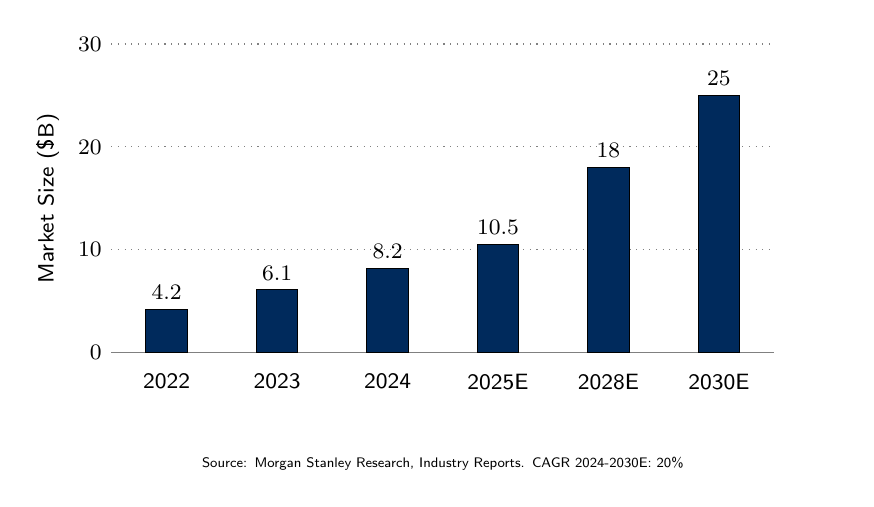
\begin{tikzpicture}
\begin{axis}[
    msstyle,
    width=10cm,
    height=5.5cm,
    symbolic x coords={2022, 2023, 2024, 2025E, 2028E, 2030E},
    xtick=data,
    xticklabel style={font=\footnotesize},
    ylabel={Market Size (\$B)},
    ylabel style={font=\footnotesize},
    yticklabel style={font=\footnotesize},
    nodes near coords,
    nodes near coords style={font=\footnotesize\bfseries, color=black, anchor=south},
    bar width=15pt,
    ymin=0, ymax=30
]
\addplot[fill=msblue] coordinates {(2022,4.2) (2023,6.1) (2024,8.2) (2025E,10.5) (2028E,18.0) (2030E,25.0)};
\end{axis}
\node[anchor=north, font=\tiny, text width=10cm, align=center] 
    at (current axis.south) [yshift=-1.2cm] {
        Source: Morgan Stanley Research, Industry Reports. CAGR 2024-2030E: 20\%
    };
\end{tikzpicture}
\end{center}

\end{multicols}

\section{siRNA Mechanism \& Therapeutic Landscape}

Small interfering RNA (siRNA) therapeutics represent a paradigm shift in drug development, enabling the precise silencing of disease-causing genes at the mRNA level. Unlike traditional small molecules that target proteins, siRNA intervenes upstream in the central dogma of biology, preventing the translation of pathogenic proteins entirely. This mechanism offers several structural advantages: \textbf{(1)} higher target specificity, \textbf{(2)} applicability to ``undruggable'' targets, and \textbf{(3)} durable effects lasting weeks to months per dose.

\subsection{The Science of Gene Silencing}

RNA interference (RNAi) is a natural cellular process discovered by Fire and Mello (Nobel Prize, 2006). siRNA molecules are synthetic double-stranded RNA sequences (typically 21-23 nucleotides) designed to target specific mRNA transcripts.

\begin{itemize}
    \item \textbf{RISC Loading:} The siRNA is loaded into the RNA-induced silencing complex (RISC), where the ``guide strand'' directs the complex to the complementary mRNA target.
    \item \textbf{mRNA Cleavage:} Argonaute-2 (Ago2), the catalytic core of RISC, cleaves the target mRNA, preventing protein synthesis.
    \item \textbf{Catalytic Turnover:} A single siRNA-RISC complex can cleave multiple mRNA copies, providing amplified therapeutic effect.
\end{itemize}

The key challenge historically was \textbf{delivery}: naked siRNA is rapidly degraded by nucleases and cannot cross cell membranes. The breakthrough came with the development of \textbf{lipid nanoparticle (LNP)} formulations (used by Onpattro) and, more importantly, \textbf{GalNAc conjugation} technology, which enables subcutaneous administration and hepatocyte-specific uptake via the asialoglycoprotein receptor (ASGPR).

\subsection{Approved siRNA Therapeutics Landscape}

The FDA has approved five siRNA therapeutics, all from Alnylam's pipeline, establishing the company as the undisputed platform leader.

\begin{table}[H]
\centering
\caption{FDA-Approved siRNA Therapeutics (2024)}
\label{tab:approved_sirna}
\tablefont
\rowcolors{2}{msgrey}{white}
\begin{adjustbox}{max width=\textwidth}
\begin{tabular}{p{0.15\textwidth}p{0.12\textwidth}p{0.18\textwidth}p{0.15\textwidth}p{0.12\textwidth}p{0.18\textwidth}}
\toprule
\rowcolor{mstableheader}
\textbf{Drug} & \textbf{Target} & \textbf{Indication} & \textbf{Approval} & \textbf{2024 Rev} & \textbf{Delivery} \\
\midrule
\textbf{Onpattro} & TTR & hATTR Polyneuropathy & Aug 2018 & \$420M & LNP (IV) \\
\textbf{Givlaari} & ALAS1 & Acute Hepatic Porphyria & Nov 2019 & \$280M & GalNAc (SC) \\
\textbf{Oxlumo} & HAO1 & Primary Hyperoxaluria & Nov 2020 & \$190M & GalNAc (SC) \\
\textbf{Amvuttra} & TTR & hATTR Polyneuropathy & Jun 2022 & \$950M & GalNAc (SC) \\
\textbf{Leqvio} & PCSK9 & Hypercholesterolemia & Dec 2021 & \$380M & GalNAc (SC) \\
\bottomrule
\end{tabular}
\end{adjustbox}
\par\vspace{0.1cm}
{\tiny Source: Company Filings, Morgan Stanley Research. Leqvio revenue reflects Novartis partnership economics.}
\end{table}

\subsection{Therapeutic Expansion: Beyond Rare Diseases}

The initial wave of siRNA approvals focused on rare diseases (hATTR amyloidosis, porphyria, hyperoxaluria) due to favorable regulatory pathways and high unmet need. However, the next decade will see expansion into \textbf{large commercial markets}:

\begin{itemize}
    \item \textbf{Cardiovascular Disease:} Leqvio (PCSK9 silencing) targets the \$15B+ LDL-lowering market. Arrowhead's Plozasiran targets elevated Lp(a), a genetically validated cardiovascular risk factor affecting 20\% of the global population.
    \item \textbf{Metabolic/NASH:} Multiple programs targeting PNPLA3, HSD17B13, and other liver-expressed genes implicated in non-alcoholic steatohepatitis.
    \item \textbf{CNS Applications:} Intrathecal delivery approaches (Alnylam's ALN-APP for Alzheimer's) represent the next frontier.
\end{itemize}

\section{Competitive Analysis: Alnylam vs. Arrowhead}

The siRNA therapeutics landscape is dominated by two pure-play companies: \textbf{Alnylam Pharmaceuticals}, the established leader with commercial products, and \textbf{Arrowhead Pharmaceuticals}, the emerging challenger with a differentiated delivery platform and cardiometabolic focus.

\subsection{Alnylam: The Platform Pioneer}

Alnylam has invested over \$10 billion in R\&D since its founding in 2002 to build the industry's most advanced RNAi platform. The company's \textbf{GalNAc conjugate technology} (marketed as Enhanced Stabilization Chemistry, ESC+) enables once-quarterly or twice-yearly subcutaneous dosing, dramatically improving patient compliance versus daily oral medications.

\textbf{Key Competitive Advantages:}
\begin{itemize}
    \item \textbf{Commercial Infrastructure:} Established US/EU sales force with rare disease expertise.
    \item \textbf{Manufacturing Scale:} Proprietary oligonucleotide synthesis at scale (Alnylam Manufacturing).
    \item \textbf{IP Moat:} Broad patent portfolio covering GalNAc chemistry, stabilization modifications, and specific sequences.
    \item \textbf{Partnership Economics:} Regeneron (CNS), Roche (ophthalmology), Novartis (Leqvio) collaborations de-risk R\&D.
\end{itemize}

\subsection{Arrowhead: The Challenger with Differentiated Delivery}

Arrowhead's \textbf{TRiM (Targeted RNAi Molecule)} platform offers potential advantages in potency and durability through proprietary ligand chemistries. While Alnylam pioneered GalNAc conjugation, Arrowhead claims its next-generation approach achieves deeper gene knockdown with extended duration.

\textbf{Key Competitive Positioning:}
\begin{itemize}
    \item \textbf{Cardiometabolic Focus:} Plozasiran (Lp(a)), ARO-APOC3 (triglycerides) target large patient populations.
    \item \textbf{Pulmonary Delivery:} ARO-MUC5AC for COPD/asthma represents potential first-in-class for lung-targeted RNAi.
    \item \textbf{Partnership Validation:} Johnson \& Johnson (JNJ-3989 for HBV), Takeda collaborations.
\end{itemize}

\begin{center}
\captionof{figure}{Revenue Trajectory: Alnylam vs. Arrowhead (\$M)}
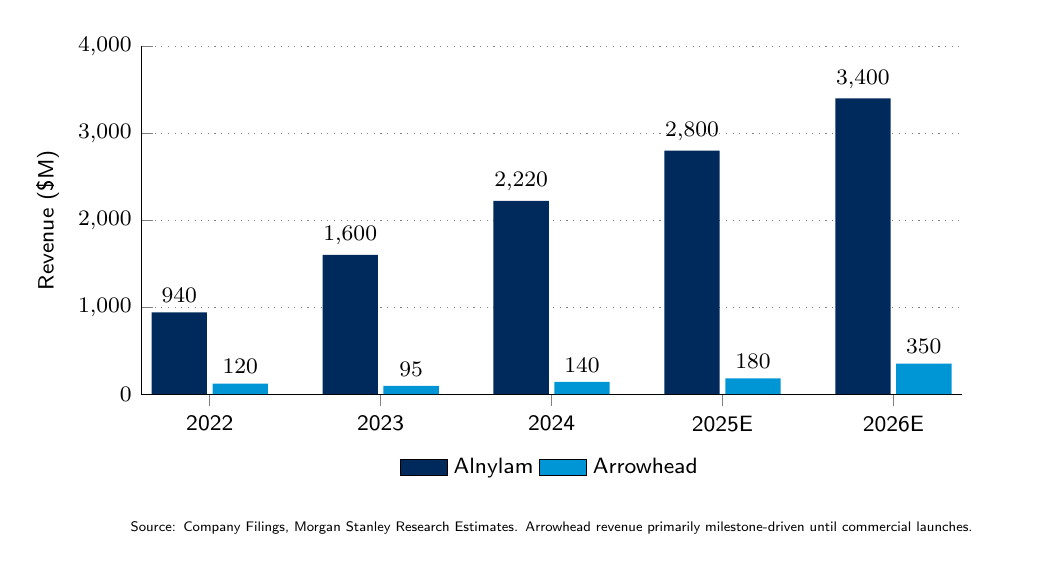
\begin{tikzpicture}
\begin{axis}[
    ybar,
    width=12cm,
    height=6cm,
    symbolic x coords={2022, 2023, 2024, 2025E, 2026E},
    xtick=data,
    xticklabel style={font=\footnotesize},
    ylabel={Revenue (\$M)},
    ylabel style={font=\footnotesize},
    yticklabel style={font=\footnotesize},
    nodes near coords,
    nodes near coords style={font=\footnotesize, color=black},
    bar width=20pt,
    ymin=0, ymax=4000,
    legend style={at={(0.5,-0.15)}, anchor=north, legend columns=-1, draw=none, font=\footnotesize},
    ymajorgrids=true,
    grid style={dotted, gray},
    axis y line*=left,
    axis x line*=bottom,
    cycle list={
        {fill=msblue, draw=none},
        {fill=msbrightblue, draw=none},
    }
]
\addplot coordinates {(2022,940) (2023,1600) (2024,2220) (2025E,2800) (2026E,3400)};
\addlegendentry{Alnylam}
\addplot coordinates {(2022,120) (2023,95) (2024,140) (2025E,180) (2026E,350)};
\addlegendentry{Arrowhead}
\end{axis}
\node[anchor=north, font=\tiny, text width=12cm, align=center] 
    at (current axis.south) [yshift=-1.5cm] {
        Source: Company Filings, Morgan Stanley Research Estimates. Arrowhead revenue primarily milestone-driven until commercial launches.
    };
\end{tikzpicture}
\end{center}

\begin{table}[H]
\centering
\caption{Competitive Platform Comparison: Alnylam vs. Arrowhead}
\label{tab:platform_comparison}
\tablefont
\rowcolors{2}{msgrey}{white}
\begin{adjustbox}{max width=\textwidth}
\begin{tabular}{p{0.22\textwidth}p{0.35\textwidth}p{0.35\textwidth}}
\toprule
\rowcolor{mstableheader}
\textbf{Dimension} & \textbf{Alnylam (ESC+)} & \textbf{Arrowhead (TRiM)} \\
\midrule
\textbf{Delivery Technology} & GalNAc conjugate (2nd gen) & Enhanced GalNAc (3rd gen claims) \\
\textbf{Dosing Frequency} & Quarterly to Semi-annual & Similar; claims longer duration \\
\textbf{Target Tissues} & Liver (proven), CNS (emerging) & Liver, Lung (novel), Muscle (preclinical) \\
\textbf{Manufacturing} & Proprietary, scaled & Partner-dependent (CMO) \\
\textbf{Commercial Stage} & 5 approved products & 0 (Phase 3 assets) \\
\textbf{IP Position} & Broad foundational patents & Freedom-to-operate; differentiated chemistry \\
\textbf{Partnership Strategy} & Selective (Regeneron, Novartis) & Aggressive (J\&J, Takeda, GSK) \\
\bottomrule
\end{tabular}
\end{adjustbox}
\par\vspace{0.1cm}
{\tiny Source: Company Presentations, Morgan Stanley Research Analysis}
\end{table}

\section{Market Size \& Growth Projections}

The global siRNA therapeutics market is experiencing exponential growth, driven by expanding indications, improved delivery technologies, and increasing adoption by prescribers. Our analysis projects the market will grow from \textbf{\$8.2 billion} in 2024 to \textbf{\$25 billion} by 2030, representing a \textbf{20\% CAGR}.

\subsection{Market Drivers}

\begin{enumerate}
    \item \textbf{Label Expansions:} Amvuttra's potential expansion into ATTR cardiomyopathy (HELIOS-B trial) could more than double its addressable market from \$3B to \$8B+.
    \item \textbf{New Indications:} Cardiovascular (Lp(a), triglycerides), metabolic (NASH), and CNS (Alzheimer's) represent multi-billion dollar opportunities.
    \item \textbf{Manufacturing Cost Reductions:} Scale-up of oligonucleotide synthesis is reducing COGS, improving margins from $\sim$20\% to projected 70\%+ at maturity.
    \item \textbf{Competitive Dynamics:} Large pharma entries (Novartis, Roche, AstraZeneca) validate the modality and accelerate market development.
\end{enumerate}

\subsection{Segment Analysis}

\begin{table}[H]
\centering
\caption{siRNA Market Segmentation by Therapeutic Area (2024 vs. 2030E)}
\label{tab:market_segments}
\tablefont
\rowcolors{2}{msgrey}{white}
\begin{adjustbox}{max width=\textwidth}
\begin{tabular}{p{0.25\textwidth}ccp{0.35\textwidth}}
\toprule
\rowcolor{mstableheader}
\textbf{Therapeutic Area} & \textbf{2024 (\$B)} & \textbf{2030E (\$B)} & \textbf{Key Drivers} \\
\midrule
\textbf{Rare Genetic (hATTR, AHP)} & 2.1 & 5.5 & Amvuttra conversion; geographic expansion \\
\textbf{Cardiovascular (PCSK9, Lp(a))} & 0.8 & 8.0 & Leqvio uptake; Plozasiran launch \\
\textbf{Hepatic (HBV, NASH)} & 0.4 & 4.5 & JNJ-3989; PNPLA3 programs \\
\textbf{Metabolic (Hyperoxaluria, etc.)} & 0.3 & 1.5 & Oxlumo growth; new indications \\
\textbf{CNS \& Other} & 0.1 & 2.5 & Intrathecal delivery advances \\
\textbf{Other/Emerging} & 4.5 & 3.0 & Generic/biosimilar pressure on older assets \\
\midrule
\textbf{Total Market} & \textbf{8.2} & \textbf{25.0} & CAGR: 20\% \\
\bottomrule
\end{tabular}
\end{adjustbox}
\par\vspace{0.1cm}
{\tiny Source: Morgan Stanley Research Estimates, Industry Analysis}
\end{table}

\begin{center}
\captionof{figure}{siRNA Market Share by Therapeutic Area (2030E)}
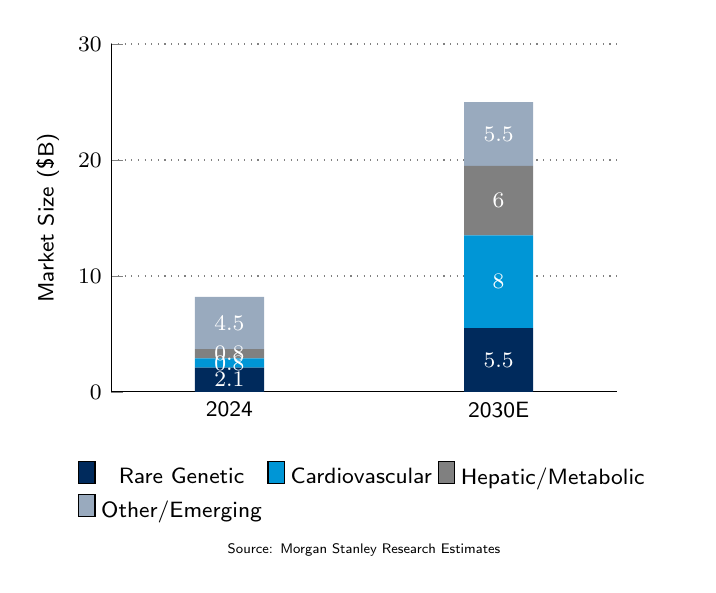
\begin{tikzpicture}
\begin{axis}[
    ybar stacked,
    width=8cm,
    height=6cm,
    bar width=25pt,
    enlarge x limits={abs=1.5cm},
    symbolic x coords={2024, 2030E},
    xtick=data,
    xticklabel style={font=\footnotesize},
    ylabel={Market Size (\$B)},
    ylabel style={font=\footnotesize},
    yticklabel style={font=\footnotesize},
    ymin=0, ymax=30,
    legend style={at={(0.5,-0.18)}, anchor=north, legend columns=3, draw=none, font=\footnotesize},
    ymajorgrids=true,
    grid style={dotted, gray},
    axis y line*=left,
    axis x line*=bottom,
    nodes near coords,
    nodes near coords style={font=\footnotesize\bfseries, color=white},
    every node near coord/.append style={anchor=center},
    cycle list={
        {fill=msblue, draw=none},
        {fill=msbrightblue, draw=none},
        {fill=gray, draw=none},
        {fill=msblue!40, draw=none},
    }
]
\addplot coordinates {(2024,2.1) (2030E,5.5)};
\addlegendentry{Rare Genetic}
\addplot coordinates {(2024,0.8) (2030E,8.0)};
\addlegendentry{Cardiovascular}
\addplot coordinates {(2024,0.8) (2030E,6.0)};
\addlegendentry{Hepatic/Metabolic}
\addplot coordinates {(2024,4.5) (2030E,5.5)};
\addlegendentry{Other/Emerging}
\end{axis}
\node[anchor=north, font=\tiny, text width=8cm, align=center] 
    at (current axis.south) [yshift=-1.8cm] {
        Source: Morgan Stanley Research Estimates
    };
\end{tikzpicture}
\end{center}

\section{Clinical Pipeline Assessment}

The siRNA therapeutics pipeline has matured significantly, with multiple Phase 3 programs across both Alnylam and Arrowhead expected to report data in 2025-2026. Our analysis identifies key catalysts and assigns probability-weighted valuations.

\subsection{Alnylam Pipeline Highlights}

\begin{itemize}
    \item \textbf{Vutrisiran (HELIOS-B):} Phase 3 trial in ATTR cardiomyopathy completed enrollment (655 patients). Primary endpoint: all-cause mortality and CV events. Readout expected H1 2025. Positive data would expand TAM by \$5B+.
    \item \textbf{ALN-APP:} Intrathecal siRNA for early-onset Alzheimer's (APP gene). Phase 1 dose-escalation ongoing. First CNS-targeted siRNA with disease-modifying potential.
    \item \textbf{Zilebesiran:} Once-quarterly hypertension treatment (angiotensinogen silencing). Phase 2 data showed 10-15 mmHg sustained BP reduction. Phase 3 initiation expected 2025.
\end{itemize}

\subsection{Arrowhead Pipeline Highlights}

\begin{itemize}
    \item \textbf{Plozasiran:} Phase 3 PALISADE trial in elevated Lp(a). First siRNA for Lp(a) lowering. Phase 2 showed 94\% Lp(a) reduction sustained for 6+ months. Registrational data expected H2 2025.
    \item \textbf{ARO-APOC3:} Phase 3 in severe hypertriglyceridemia. Potential best-in-class with 90\%+ TG reduction. Partnership discussions ongoing.
    \item \textbf{ARO-MUC5AC:} First inhaled siRNA for COPD. Phase 1/2 initiated. If successful, opens lung delivery as new tissue target.
\end{itemize}

\begin{table}[H]
\centering
\caption{Key Clinical Catalysts: 2025-2026}
\label{tab:catalysts}
\tablefont
\rowcolors{2}{msgrey}{white}
\begin{adjustbox}{max width=\textwidth}
\begin{tabular}{p{0.18\textwidth}p{0.12\textwidth}p{0.18\textwidth}p{0.12\textwidth}p{0.30\textwidth}}
\toprule
\rowcolor{mstableheader}
\textbf{Asset} & \textbf{Company} & \textbf{Indication} & \textbf{Timing} & \textbf{Significance} \\
\midrule
\textbf{Vutrisiran} & Alnylam & ATTR-CM & H1 2025 & \$5B+ TAM expansion; survival endpoint \\
\textbf{Plozasiran} & Arrowhead & Elevated Lp(a) & H2 2025 & First-in-class; CV outcomes potential \\
\textbf{Zilebesiran} & Alnylam & Hypertension & 2025-2026 & \$50B+ HTN market entry \\
\textbf{ARO-APOC3} & Arrowhead & Hypertriglyceridemia & 2025 & Best-in-class TG lowering \\
\textbf{JNJ-3989} & J\&J/Arrowhead & Chronic HBV & 2026 & Functional cure potential \\
\bottomrule
\end{tabular}
\end{adjustbox}
\par\vspace{0.1cm}
{\tiny Source: Company Pipelines, ClinicalTrials.gov, Morgan Stanley Research}
\end{table}

\subsection{Clinical Trial Success Rate Analysis}

siRNA therapeutics have demonstrated higher clinical success rates compared to traditional small molecules, driven by the precision of target engagement and the ability to validate knockdown pharmacodynamically.

\begin{center}
\captionof{figure}{Clinical Trial Success Rates by Modality (\%)}
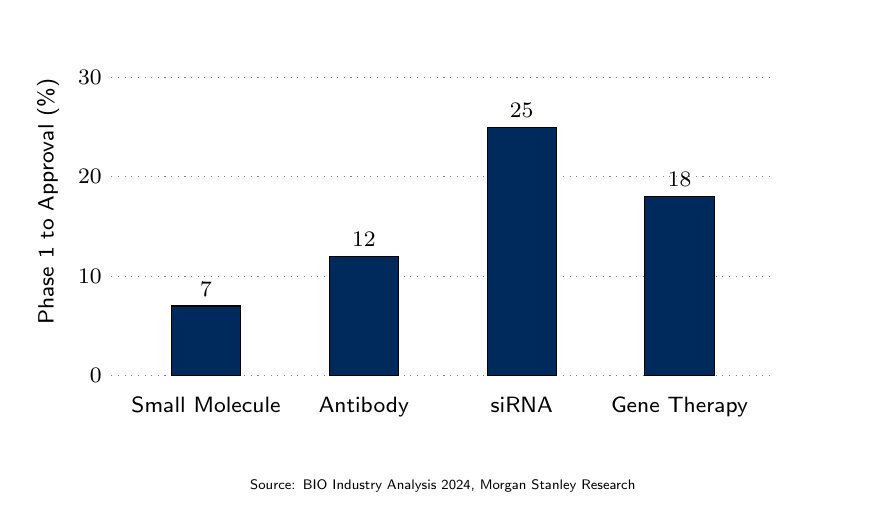
\begin{tikzpicture}
\begin{axis}[
    comparestyle,
    width=10cm,
    height=6cm,
    symbolic x coords={Small Molecule, Antibody, siRNA, Gene Therapy},
    xtick=data,
    xticklabel style={font=\footnotesize},
    ylabel={Phase 1 to Approval (\%)},
    ylabel style={font=\footnotesize},
    yticklabel style={font=\footnotesize},
    nodes near coords,
    nodes near coords style={font=\footnotesize\bfseries, color=black},
    bar width=25pt,
    ymin=0, ymax=35,
    enlarge x limits=0.2
]
\addplot[fill=msblue] coordinates {(Small Molecule,7) (Antibody,12) (siRNA,25) (Gene Therapy,18)};
\end{axis}
\node[anchor=north, font=\tiny, text width=10cm, align=center] 
    at (current axis.south) [yshift=-1.2cm] {
        Source: BIO Industry Analysis 2024, Morgan Stanley Research
    };
\end{tikzpicture}
\end{center}

\section{Investment Risks}

\subsection{Platform-Specific Risks}

\begin{itemize}
    \item \textbf{Delivery Limitations:} Current GalNAc technology is liver-restricted. Extra-hepatic delivery (muscle, CNS, lung) remains challenging. Failure to expand tissue targeting would limit TAM growth.
    \item \textbf{Immunogenicity:} Long-term repeated dosing may trigger anti-drug antibodies. Limited long-term safety data beyond 5 years.
    \item \textbf{Manufacturing Complexity:} Oligonucleotide synthesis requires specialized capabilities. Supply chain concentration risk (few qualified CMOs).
\end{itemize}

\subsection{Company-Specific Risks}

\textbf{Alnylam:}
\begin{itemize}
    \item \textbf{HELIOS-B Binary Risk:} Negative trial would significantly impact valuation (20-30\% downside).
    \item \textbf{Partnership Concentration:} Novartis economics on Leqvio limit upside capture.
    \item \textbf{Competition:} Ionis antisense programs, emerging siRNA players (Dicerna/Novo, Silence Therapeutics).
\end{itemize}

\textbf{Arrowhead:}
\begin{itemize}
    \item \textbf{Execution Risk:} No approved products; reliant on clinical success for valuation.
    \item \textbf{Cash Runway:} \$650M cash supports operations through 2026, but Phase 3 costs may require additional financing.
    \item \textbf{Plozasiran Uncertainty:} Lp(a) lowering is pharmacodynamically validated, but CV outcomes benefit unproven.
\end{itemize}

\subsection{Competitive and Regulatory Risks}

\begin{itemize}
    \item \textbf{Biosimilar/Generic Entry:} Onpattro faces potential competition post-2028 as patents expire.
    \item \textbf{Pricing Pressure:} IRA drug pricing provisions may impact siRNA economics in Medicare populations.
    \item \textbf{Regulatory Scrutiny:} Novel modality may face heightened post-market surveillance requirements.
\end{itemize}

\begin{table}[H]
\centering
\caption{Risk Matrix: siRNA Investment Considerations}
\label{tab:risk_matrix}
\tablefont
\rowcolors{2}{msgrey}{white}
\begin{adjustbox}{max width=\textwidth}
\begin{tabular}{p{0.25\textwidth}p{0.12\textwidth}p{0.12\textwidth}p{0.45\textwidth}}
\toprule
\rowcolor{mstableheader}
\textbf{Risk Factor} & \textbf{Probability} & \textbf{Impact} & \textbf{Mitigant/Monitoring} \\
\midrule
\textbf{HELIOS-B Failure} & 25\% & Critical & Pre-specified interim analysis; prior Onpattro efficacy \\
\textbf{Plozasiran Ph3 Miss} & 35\% & High & Strong Ph2 data; genetic validation of Lp(a) \\
\textbf{Manufacturing Disruption} & 15\% & Moderate & Dual-source strategy; inventory buffers \\
\textbf{Competitive Encroachment} & 40\% & Moderate & IP protection; first-mover advantage \\
\textbf{Pricing/Reimbursement} & 30\% & Moderate & Rare disease orphan status; outcomes data \\
\bottomrule
\end{tabular}
\end{adjustbox}
\par\vspace{0.1cm}
{\tiny Source: Morgan Stanley Research Risk Assessment}
\end{table}

\subsection{Investment Recommendation Summary}

\begin{multicols}{2}

\textbf{Alnylam (ALNY) --- OVERWEIGHT}

Our \$285 price target implies 25\% upside from current levels. The investment case rests on:
\begin{itemize}
    \item Commercial momentum: Amvuttra trajectory to \$1.5B+ by 2026
    \item Pipeline optionality: HELIOS-B, zilebesiran catalysts
    \item Platform leadership: GalNAc IP moat
    \item Balance sheet strength: \$2.1B cash, no near-term dilution risk
\end{itemize}

\textbf{Key Risk:} Binary HELIOS-B outcome in H1 2025.

\columnbreak

\textbf{Arrowhead (ARWR) --- EQUAL-WEIGHT}

Our \$38 price target reflects risk-adjusted pipeline NPV. The investment case balances:
\begin{itemize}
    \item Upside: Plozasiran first-in-class potential; TRiM platform differentiation
    \item Downside: Clinical execution risk; cash runway concerns; no commercial infrastructure
\end{itemize}

We would upgrade to OVERWEIGHT on positive Plozasiran Phase 3 data demonstrating $>$80\% Lp(a) reduction with clean safety profile.

\textbf{Key Risk:} Plozasiran binary event H2 2025.

\end{multicols}

\vspace{0.5cm}

\begin{center}
\begin{tcolorbox}[colback=msgrey, colframe=msblue, boxrule=1pt, sharp corners, width=0.9\textwidth]
\textbf{\color{msblue}Investment Conclusion:} siRNA therapeutics represent a generational investment opportunity in precision medicine. Alnylam offers de-risked exposure to the platform's maturation, while Arrowhead provides leveraged upside for risk-tolerant investors. We recommend portfolio allocation weighted toward Alnylam (70\%) with tactical Arrowhead exposure (30\%) ahead of key 2025 catalysts.
\end{tcolorbox}
\end{center}

\end{document}
